%==============================================================
% TI EdgeAI Model Zoo — Detailed Slide Deck
% LaTeX Beamer Presentation
% Version 11.2.0 | August 2026
%==============================================================

\documentclass[aspectratio=169,12pt]{beamer}

%--------------------------------------------------------------
% Theme & Colors
%--------------------------------------------------------------
\usetheme{Madrid}
\usecolortheme{default}

% TI brand colors
\definecolor{TIRed}{RGB}{200,16,46}
\definecolor{TIDark}{RGB}{58,58,58}
\definecolor{TIBlue}{RGB}{0,114,188}
\definecolor{TIGray}{RGB}{237,237,237}
\definecolor{TIGreen}{RGB}{0,153,68}
\definecolor{TIOrange}{RGB}{244,124,32}
\definecolor{TILightBlue}{RGB}{0,163,224}

\setbeamercolor{palette primary}{bg=TIRed,fg=white}
\setbeamercolor{palette secondary}{bg=TIDark,fg=white}
\setbeamercolor{palette tertiary}{bg=TIBlue,fg=white}
\setbeamercolor{palette quaternary}{bg=TIDark,fg=white}
\setbeamercolor{structure}{fg=TIRed}
\setbeamercolor{section in toc}{fg=TIDark}
\setbeamercolor{alerted text}{fg=TIRed}
\setbeamercolor{block title}{bg=TIBlue,fg=white}
\setbeamercolor{block body}{bg=TIGray,fg=TIDark}
\setbeamercolor{block title alerted}{bg=TIRed,fg=white}
\setbeamercolor{block body alerted}{bg=TIGray,fg=TIDark}
\setbeamercolor{block title example}{bg=TIGreen,fg=white}
\setbeamercolor{block body example}{bg=TIGray,fg=TIDark}

%--------------------------------------------------------------
% Packages
%--------------------------------------------------------------
\usepackage{booktabs}
\usepackage{graphicx}
\usepackage{tikz}
\usepackage{pgfplots}
\pgfplotsset{compat=1.18}
\usepackage{array}
\usepackage{colortbl}
\usepackage{xcolor}
\usepackage{fontawesome5}
\usepackage{listings}
\usepackage{multicol}
\usepackage{tcolorbox}
\usepackage{amsmath}
\usepackage{hyperref}

\usetikzlibrary{shapes.geometric, arrows.meta, positioning, fit, backgrounds,
                decorations.pathmorphing, matrix, calc, shadows}

%--------------------------------------------------------------
% Custom Commands
%--------------------------------------------------------------
\newcommand{\highlight}[1]{\textcolor{TIRed}{\textbf{#1}}}
\newcommand{\blue}[1]{\textcolor{TIBlue}{\textbf{#1}}}
\newcommand{\green}[1]{\textcolor{TIGreen}{\textbf{#1}}}

\newcommand{\taskbadge}[2]{%
  \tikz[baseline=-0.5ex]\node[rounded corners=3pt, fill=#1, text=white,
    font=\tiny\bfseries, inner sep=2pt]{#2};%
}

%--------------------------------------------------------------
% Metadata
%--------------------------------------------------------------
\title[TI EdgeAI Model Zoo]{\textbf{Texas Instruments EdgeAI Model Zoo}}
\subtitle{Comprehensive Technical Overview --- Version 11.2.0}
\author{TI Edge AI Engineering}
\institute{Texas Instruments Inc.}
\date{August 2026}

\logo{\tikz\node[inner sep=0]{\textcolor{TIRed}{\textbf{TI}}~EdgeAI};}

%==============================================================
\begin{document}
%==============================================================

%--------------------------------------------------------------
% TITLE SLIDE
%--------------------------------------------------------------
\begin{frame}[plain]
  
\begin{tikzpicture}[remember picture, overlay]
    % Background gradient
    \fill[TIDark] (current page.south west) rectangle (current page.north east);
    \fill[TIRed, opacity=0.85]
      (current page.south west) rectangle
      ([yshift=2.5cm]current page.south east);
    % Decorative diagonal stripe
    \fill[TIBlue, opacity=0.3]
      ([xshift=-1cm]current page.north west) --
      ([xshift=6cm]current page.north west) --
      ([xshift=4cm]current page.south west) --
      ([xshift=-1cm]current page.south west) -- cycle;
  \end{tikzpicture}

  \vspace{0.8cm}
  \begin{center}
    {\color{white}\Huge\textbf{TI EdgeAI Model Zoo}}\\[0.3cm]
    {\color{TIGray}\large Comprehensive Technical Overview}\\[0.1cm]
    {\color{TIGray}\normalsize Version 11.2.0}\\[0.8cm]
    
\begin{tikzpicture}
      \node[rounded corners=6pt, fill=TIRed, text=white, inner sep=8pt,
            font=\footnotesize]{
        \faServer~\textbf{5 SoC Families} \quad
        \faLayerGroup~\textbf{8 Vision Tasks} \quad
        \faDatabase~\textbf{180+ Models} \quad
        \faCode~\textbf{ONNX + TFLite}
      };
    \end{tikzpicture}\\[0.6cm]
    {\color{TIGray}\small Texas Instruments Inc.\ $\cdot$ August 2026}
  \end{center}
\end{frame}

%--------------------------------------------------------------
% AGENDA
%--------------------------------------------------------------
\begin{frame}{Agenda}
  \begin{columns}[T]
    \begin{column}{0.48\textwidth}
      \tableofcontents[sections={1-6}]
    \end{column}
    \begin{column}{0.48\textwidth}
      \tableofcontents[sections={7-11}]
    \end{column}
  \end{columns}
\end{frame}

%==============================================================
\section{Overview}
%==============================================================

\begin{frame}{What is the TI EdgeAI Model Zoo?}
  \begin{columns}[T]
    \begin{column}{0.56\textwidth}
      \begin{block}{Definition}
        A curated collection of \highlight{180+ pre-trained DNN models} for
        embedded computer vision, optimized for TI's AI-capable SoCs.
      \end{block}

      \vspace{0.4cm}
      \textbf{Core objectives:}
      \begin{itemize}
        \item Ready-to-deploy baselines for \blue{8 vision tasks}
        \item Embedded-friendly formats (ONNX, TFLite) for TIDL compilation
        \item \highlight{Pre-compiled INT8 artifacts} for 5 TI SoC families
        \item ``Lite'' architectural variants optimized for edge hardware
        \item INT8 quantization aligned with TI's MMA/C7x accelerators
      \end{itemize}

      \vspace{0.3cm}
      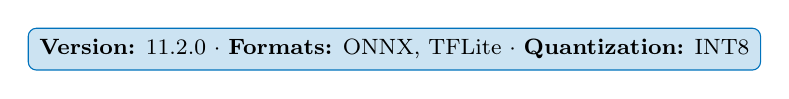
\begin{tikzpicture}
        \node[rounded corners=3pt, fill=TIBlue!20, draw=TIBlue, inner sep=4pt,
              font=\footnotesize]{
          \textbf{Version:} 11.2.0 $\cdot$
          \textbf{Formats:} ONNX, TFLite $\cdot$
          \textbf{Quantization:} INT8
        };
      \end{tikzpicture}
    \end{column}

    \begin{column}{0.40\textwidth}
      \begin{tikzpicture}[scale=0.78, every node/.style={font=\scriptsize}]
        % Target applications box
        \node[rounded corners=5pt, fill=TIRed!15, draw=TIRed,
              minimum width=5.2cm, minimum height=4.2cm,
              label={[TIRed, font=\small\bfseries]north:Target Applications}]
              (apps) at (0,0) {};

        \node[fill=TIRed, text=white, rounded corners=3pt,
              inner sep=3pt, font=\scriptsize\bfseries] at (-1.2, 1.3)
              {\faCarSide~Automotive};
        \node[fill=TIBlue, text=white, rounded corners=3pt,
              inner sep=3pt, font=\scriptsize\bfseries] at (1.1, 1.3)
              {\faIndustry~Industrial};
        \node[fill=TIGreen, text=white, rounded corners=3pt,
              inner sep=3pt, font=\scriptsize\bfseries] at (-1.1, 0.2)
              {\faRobot~Robotics};
        \node[fill=TIOrange, text=white, rounded corners=3pt,
              inner sep=3pt, font=\scriptsize\bfseries] at (1.1, 0.2)
              {\faCamera~Surveillance};
        \node[fill=TIDark, text=white, rounded corners=3pt,
              inner sep=3pt, font=\scriptsize\bfseries] at (0, -0.9)
              {\faMicrochip~Embedded AI};
      \end{tikzpicture}
    \end{column}
  \end{columns}
\end{frame}

%--------------------------------------------------------------
\begin{frame}{Repository Structure}
  \begin{columns}[T]
    \begin{column}{0.52\textwidth}
      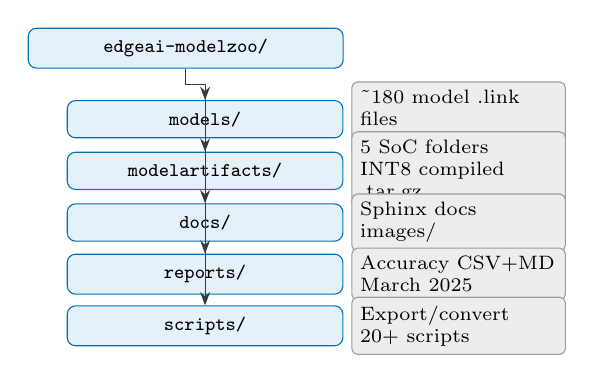
\begin{tikzpicture}[scale=0.82,
        dir/.style={draw=TIBlue, fill=TIBlue!10, rounded corners=3pt,
                    inner sep=4pt, font=\ttfamily\scriptsize},
        file/.style={draw=TIDark!50, fill=TIGray, rounded corners=2pt,
                     inner sep=3pt, font=\ttfamily\scriptsize},
        arr/.style={->, >=Stealth, TIDark, thin}
      ]
        \node[dir, minimum width=4cm] (root) at (0,4.0) {edgeai-modelzoo/};
        \node[dir, minimum width=3.5cm] (models) at (0.3,2.9) {models/};
        \node[dir, minimum width=3.5cm] (artifacts) at (0.3,2.1) {modelartifacts/};
        \node[dir, minimum width=3.5cm] (docs) at (0.3,1.3) {docs/};
        \node[dir, minimum width=3.5cm] (reports) at (0.3,0.5) {reports/};
        \node[dir, minimum width=3.5cm] (scripts) at (0.3,-0.3) {scripts/};

        \draw[arr] (root.south) -- ++(0,-0.25) -| (models.north);
        \draw[arr] (root.south) -- ++(0,-0.25) -| (artifacts.north);
        \draw[arr] (root.south) -- ++(0,-0.25) -| (docs.north);
        \draw[arr] (root.south) -- ++(0,-0.25) -| (reports.north);
        \draw[arr] (root.south) -- ++(0,-0.25) -| (scripts.north);

        \node[file, right=0.1cm of models, font=\scriptsize, text width=2.5cm]
          {\textasciitilde{}180 model .link files\\ 8 vision task folders};
        \node[file, right=0.1cm of artifacts, font=\scriptsize, text width=2.5cm]
          {5 SoC folders\\ INT8 compiled .tar.gz};
        \node[file, right=0.1cm of docs, font=\scriptsize, text width=2.5cm]
          {Sphinx docs\\ images/};
        \node[file, right=0.1cm of reports, font=\scriptsize, text width=2.5cm]
          {Accuracy CSV+MD\\ March 2025};
        \node[file, right=0.1cm of scripts, font=\scriptsize, text width=2.5cm]
          {Export/convert\\ 20+ scripts};
      \end{tikzpicture}
    \end{column}

    \begin{column}{0.44\textwidth}
      \begin{alertblock}{Key Design: .link Files}
        Model binaries are \textbf{NOT stored in Git}.\\
        \texttt{.link} files contain hosted download URLs.\\
        Run \texttt{run\_download\_modelartifacts.sh} to fetch compiled artifacts.
      \end{alertblock}

      \vspace{0.3cm}
      \begin{exampleblock}{models/ Sub-structure}
        \begin{itemize}\scriptsize
          \item \texttt{vision/classification/}
          \item \texttt{vision/detection/}
          \item \texttt{vision/segmentation/}
          \item \texttt{vision/depth\_estimation/}
          \item \texttt{vision/detection\_3d/}
          \item \texttt{vision/keypoint/}
          \item \texttt{vision/object\_6d\_pose/}
          \item \texttt{vision/visual\_localization/}
          \item \texttt{model\_infos.py} — full metadata dict
          \item \texttt{configs.yaml} — config file map
        \end{itemize}
      \end{exampleblock}
    \end{column}
  \end{columns}
\end{frame}

%==============================================================
\section{Supported Hardware}
%==============================================================

\begin{frame}{TI SoC Target Hardware}
  \begin{center}
  \begin{tikzpicture}[scale=0.88,
    soc/.style={rounded corners=6pt, minimum width=2.5cm, minimum height=2.2cm,
                draw, thick, align=center, font=\small\bfseries},
    label/.style={font=\scriptsize, align=center}
  ]
    % TDA4VM
    \node[soc, fill=TIRed!20, draw=TIRed] (tda) at (-5.5, 0)
      {\textcolor{TIRed}{TDA4VM}\\[2pt]
       \scriptsize Jacinto 7\\
       \scriptsize Automotive};

    % AM62A
    \node[soc, fill=TIBlue!15, draw=TIBlue] (am62) at (-2.75, 0)
      {\textcolor{TIBlue}{AM62A}\\[2pt]
       \scriptsize Entry AI\\
       \scriptsize Industrial};

    % AM67A
    \node[soc, fill=TIBlue!20, draw=TIBlue!70] (am67) at (0, 0)
      {\textcolor{TIBlue!80}{AM67A}\\[2pt]
       \scriptsize Mid-Range\\
       \scriptsize AI SoC};

    % AM68A
    \node[soc, fill=TIGreen!15, draw=TIGreen] (am68) at (2.75, 0)
      {\textcolor{TIGreen}{AM68A}\\[2pt]
       \scriptsize High Perf.\\
       \scriptsize Benchmark};

    % AM69A
    \node[soc, fill=TIOrange!15, draw=TIOrange] (am69) at (5.5, 0)
      {\textcolor{TIOrange}{AM69A}\\[2pt]
       \scriptsize Top-Tier\\
       \scriptsize Multi-Camera};

    % Common INT8 label
    \node[rounded corners=4pt, fill=TIDark, text=white,
          minimum width=12cm, inner sep=5pt, font=\small\bfseries]
          at (0, -1.8) {All 5 SoCs: INT8 Quantized Artifacts Available};

    % Application labels
    \node[label, text=TIRed] at (-5.5, 1.6)
      {\faCarSide\\ADAS \& Drive Assist};
    \node[label, text=TIBlue] at (-2.75, 1.6)
      {\faIndustry\\Embedded Edge};
    \node[label, text=TIBlue!80] at (0, 1.6)
      {\faThLarge\\Balanced};
    \node[label, text=TIGreen] at (2.75, 1.6)
      {\faTachometerAlt\\Reference Eval};
    \node[label, text=TIOrange] at (5.5, 1.6)
      {\faServer\\High Throughput};

    % Performance arrow
    \draw[->, very thick, TIDark!60, dashed]
      ([yshift=-0.6cm]tda.east) -- ([yshift=-0.6cm]am69.west)
      node[midway, below=2pt, font=\scriptsize\itshape]{Increasing Performance →};
  \end{tikzpicture}
  \end{center}

  \vspace{0.2cm}
  \begin{columns}[T]
    \begin{column}{0.48\textwidth}
      \begin{block}{TIDL Acceleration Components}
        \begin{itemize}\footnotesize
          \item \textbf{MMA} — Matrix Multiplication Accelerator (conv, FC)
          \item \textbf{C7x DSP} — Element-wise ops, activation functions
          \item \textbf{ARM Cortex-A} — Pre/post-processing
        \end{itemize}
      \end{block}
    \end{column}
    \begin{column}{0.48\textwidth}
      \begin{alertblock}{Note on AM68A}
        \footnotesize Accuracy reports use \textbf{AM68A} as the reference
        evaluation SoC for both FP32 simulation and INT8 quantized benchmarks.
      \end{alertblock}
    \end{column}
  \end{columns}
\end{frame}

%==============================================================
\section{Model Categories Overview}
%==============================================================

\begin{frame}{Eight Supported Vision Tasks}
  \begin{tikzpicture}[scale=0.9,
    task/.style={rounded corners=5pt, minimum width=3.4cm, minimum height=1.4cm,
                 align=center, font=\small\bfseries, draw, thick, drop shadow}
  ]
    % Row 1
    \node[task, fill=TIRed!20, draw=TIRed] at (-5.0, 2.2)
      {\textcolor{TIRed}{\faImages}\\[2pt]Image\\Classification};

    \node[task, fill=TIBlue!20, draw=TIBlue] at (-1.5, 2.2)
      {\textcolor{TIBlue}{\faSearch}\\[2pt]Object\\Detection};

    \node[task, fill=TIGreen!20, draw=TIGreen] at (2.0, 2.2)
      {\textcolor{TIGreen}{\faPaintBrush}\\[2pt]Semantic\\Segmentation};

    \node[task, fill=TIOrange!20, draw=TIOrange] at (5.5, 2.2)
      {\textcolor{TIOrange}{\faCubes}\\[2pt]Depth\\Estimation};

    % Row 2
    \node[task, fill=TIDark!15, draw=TIDark!60] at (-5.0, 0.3)
      {\textcolor{TIDark}{\faCar}\\[2pt]3D Object\\Detection};

    \node[task, fill=TILightBlue!30, draw=TILightBlue!80] at (-1.5, 0.3)
      {\textcolor{TILightBlue!80}{\faRunning}\\[2pt]Keypoint\\Detection};

    \node[task, fill=TIRed!10, draw=TIRed!60] at (2.0, 0.3)
      {\textcolor{TIRed!80}{\faCube}\\[2pt]6D Pose\\Estimation};

    \node[task, fill=TIBlue!10, draw=TIBlue!60] at (5.5, 0.3)
      {\textcolor{TIBlue!70}{\faMapMarkedAlt}\\[2pt]Visual\\Localization};

    % Count badges
    \foreach \x/\y/\c/\n in {
      -5.0/2.2/TIRed/80+,
      -1.5/2.2/TIBlue/50+,
       2.0/2.2/TIGreen/30+,
       5.5/2.2/TIOrange/2,
      -5.0/0.3/TIDark/4,
      -1.5/0.3/TILightBlue/5,
       2.0/0.3/TIRed/1,
       5.5/0.3/TIBlue/1}
    {
      \node[rounded corners=2pt, fill=\c, text=white,
            font=\tiny\bfseries, inner sep=2pt] at (\x+1.4, \y+0.55) {\n~models};
    }
  \end{tikzpicture}
\end{frame}

%==============================================================
\section{Image Classification}
%==============================================================

\begin{frame}{Image Classification --- Model Landscape}
  \begin{columns}[T]
    \begin{column}{0.50\textwidth}
      \textbf{Task Setup}
      \begin{itemize}\footnotesize
        \item \textbf{Dataset:} ImageNet-1K (1000 classes, 50K val)
        \item \textbf{Input:} 224×224 RGB (most models)
        \item \textbf{Metric:} Top-1 Accuracy \%
        \item \textbf{Models:} \highlight{80+} across 10 source frameworks
      \end{itemize}

      \vspace{0.3cm}
      \textbf{Source Frameworks}
      \begin{itemize}\scriptsize
        \item edgeai-torchvision (TI PyTorch fork)
        \item edgeai-tv2 (TI newer PyTorch fork)
        \item HuggingFace Transformers (TI fork)
        \item TF-TPU (EfficientNet family)
        \item TF1/TF2 Model Garden
        \item MXNet / GluonCV
        \item Facebookresearch / pycls (RegNetX)
        \item MLPerf standardized baselines
        \item ONNX Model Zoo
        \item TIMM (timm library)
      \end{itemize}
    \end{column}

    \begin{column}{0.46\textwidth}
      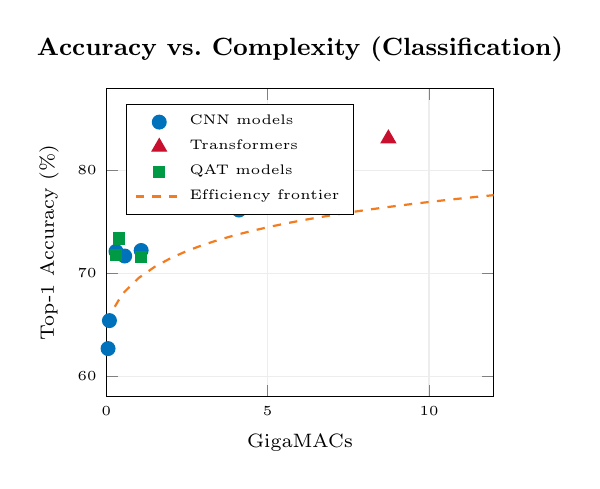
\begin{tikzpicture}
        \begin{axis}[
          title={\small Accuracy vs.\ Complexity (Classification)},
          xlabel={\scriptsize GigaMACs},
          ylabel={\scriptsize Top-1 Accuracy (\%)},
          xmin=0, xmax=12,
          ymin=58, ymax=88,
          width=6.5cm, height=5.5cm,
          grid=major, grid style={TIGray},
          tick label style={font=\tiny},
          label style={font=\scriptsize},
          title style={font=\scriptsize\bfseries},
          legend style={font=\tiny, at={(0.05,0.95)}, anchor=north west},
          legend cell align=left,
        ]
          % CNNs
          \addplot[only marks, mark=*, mark size=2.5pt, TIBlue]
            coordinates {
              (0.054, 62.68) (0.097, 65.4) (0.30, 72.13)
              (0.569, 71.68) (1.08, 72.22) (4.11, 76.15)
              (2.64, 81.5) (4.77, 82.6)
            };
          \addlegendentry{CNN models}

          % Transformers
          \addplot[only marks, mark=triangle*, mark size=3pt, TIRed]
            coordinates {
              (4.5, 81.2) (8.74, 83.1) (15.4, 84.81) (34.5, 86.15)
            };
          \addlegendentry{Transformers}

          % QAT
          \addplot[only marks, mark=square*, mark size=2pt, TIGreen]
            coordinates {
              (0.30, 71.76) (1.08, 71.61) (0.4, 73.38)
            };
          \addlegendentry{QAT models}

          % Efficiency frontier line
          \addplot[dashed, TIOrange, thick, domain=0:12]
            {68 + 3.8*ln(x+0.5)};
          \addlegendentry{Efficiency frontier};

        \end{axis}
      \end{tikzpicture}
    \end{column}
  \end{columns}
\end{frame}

%--------------------------------------------------------------
\begin{frame}{Image Classification --- Key Models Table}
  \centering
  \footnotesize
  \begin{tabular}{lrrll}
    \toprule
    \textbf{Model} & \textbf{GMACs} & \textbf{Top-1 \%} & \textbf{Format} & \textbf{Runtime} \\
    \midrule
    \rowcolor{TIGray} MobileNetV3Lite-Small & 0.054 & 62.68 & ONNX & onnxrt \\
    MobileNetV2-0.5x & 0.097 & 65.40 & ONNX & onnxrt \\
    \rowcolor{TIGray} MobileNetV1 (MLPerf) & 0.569 & 71.68 & TFLite & tflitert \\
    MobileNetV2 & 0.300 & 72.13 & ONNX & onnxrt \\
    \rowcolor{TIGray} MobileNetV2-QAT & 0.300 & 71.76 & ONNX & onnxrt \\
    MobileNetV3Lite-Large & 1.08 & 72.22 & ONNX & onnxrt \\
    \rowcolor{TIGray} ResNet18 & 1.83 & 69.76 & ONNX & onnxrt \\
    ResNet50 & 4.11 & 76.15 & ONNX & onnxrt \\
    \rowcolor{TIGray} EfficientNet-Lite4 & 2.64 & 81.50 & TFLite & tflitert \\
    EfficientNet-EdgeTPU-L & 4.77 & 82.60 & TFLite & tflitert \\
    \rowcolor{TIGray} Swin-Tiny & 4.50 & 80.43 & ONNX & onnxrt \\
    Swin-Small & 8.74 & 83.10 & ONNX & onnxrt \\
    \rowcolor{TIGray} \textbf{Swin-Large} & 34.50 & \textbf{86.15} & ONNX & onnxrt \\
    VGG16 & 15.35 & 71.59 & ONNX & onnxrt \\
    \bottomrule
  \end{tabular}

  \vspace{0.3cm}
  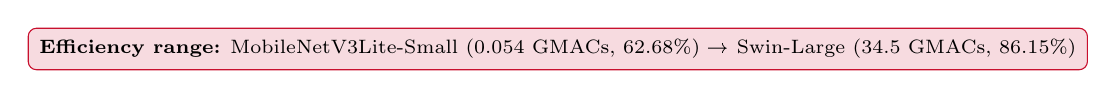
\begin{tikzpicture}
    \node[rounded corners=3pt, fill=TIRed!15, draw=TIRed, inner sep=4pt,
          font=\scriptsize]{
      \textbf{Efficiency range:}
      MobileNetV3Lite-Small (0.054 GMACs, 62.68\%) →
      Swin-Large (34.5 GMACs, 86.15\%)
    };
  \end{tikzpicture}
\end{frame}

%==============================================================
\section{Object Detection}
%==============================================================

\begin{frame}{Object Detection --- Detector Families}
  \begin{columns}[T]
    \begin{column}{0.50\textwidth}
      \textbf{Task Setup}
      \begin{itemize}\footnotesize
        \item \textbf{Dataset:} COCO 2017 (80 classes, 5K val)
        \item \textbf{Secondary:} WIDER FACE (face detection)
        \item \textbf{Metric:} mAP @ [IoU 0.5:0.95]
        \item \textbf{Models:} \highlight{50+} models
        \item \textbf{Input range:} 300px – 768px
      \end{itemize}

      \vspace{0.3cm}
      \begin{block}{Detector Architectures}
        \begin{itemize}\scriptsize
          \item \textbf{YOLOX} family (nano/tiny/s/m/l/x-lite)
          \item \textbf{YOLOv7-l} / \textbf{YOLOv9-s} (2025 additions)
          \item \textbf{RTMDet} (2025 additions)
          \item \textbf{SSD} + MobileNet/RegNetX/FPN backbones
          \item \textbf{EfficientDet-b0/b1}
          \item \textbf{FCOS} (anchor-free, r50 backbone)
          \item \textbf{CenterNet} (anchor-free, r18 backbone)
          \item \textbf{DETR} (transformer-based, r50)
        \end{itemize}
      \end{block}
    \end{column}

    \begin{column}{0.46\textwidth}
      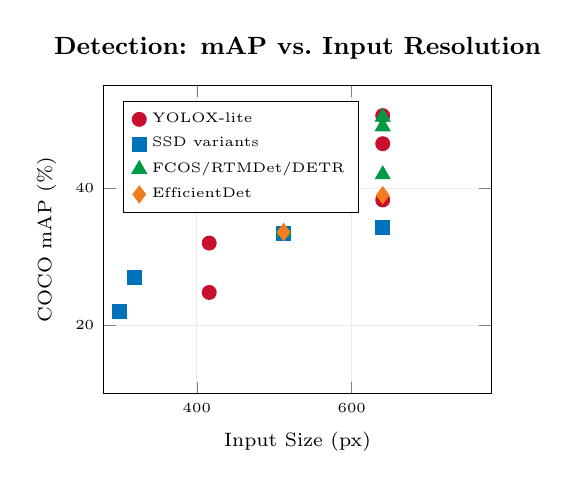
\begin{tikzpicture}
        \begin{axis}[
          title={\small Detection: mAP vs.\ Input Resolution},
          xlabel={\scriptsize Input Size (px)},
          ylabel={\scriptsize COCO mAP (\%)},
          xmin=280, xmax=780,
          ymin=10, ymax=55,
          width=6.5cm, height=5.5cm,
          grid=major, grid style={TIGray},
          tick label style={font=\tiny},
          label style={font=\scriptsize},
          title style={font=\scriptsize\bfseries},
          legend style={font=\tiny, at={(0.05,0.95)}, anchor=north west},
          legend cell align=left,
        ]
          % YOLOX family
          \addplot[only marks, mark=*, mark size=2.5pt, TIRed]
            coordinates {(416,24.8) (416,32.0) (640,38.3) (640,46.5) (640,50.6)};
          \addlegendentry{YOLOX-lite}

          % SSD family
          \addplot[only marks, mark=square*, mark size=2.5pt, TIBlue]
            coordinates {(300,22.0) (320,27.0) (512,33.4) (640,34.3)};
          \addlegendentry{SSD variants}

          % TI-lite general
          \addplot[only marks, mark=triangle*, mark size=3pt, TIGreen]
            coordinates {(512,33.6) (640,42.0) (640,49.0) (640,50.4)};
          \addlegendentry{FCOS/RTMDet/DETR}

          % EfficientDet
          \addplot[only marks, mark=diamond*, mark size=3pt, TIOrange]
            coordinates {(512,33.6) (640,39.0)};
          \addlegendentry{EfficientDet}
        \end{axis}
      \end{tikzpicture}
    \end{column}
  \end{columns}
\end{frame}

%--------------------------------------------------------------
\begin{frame}{Object Detection --- ``Lite'' Architecture Modifications}
  \begin{center}
  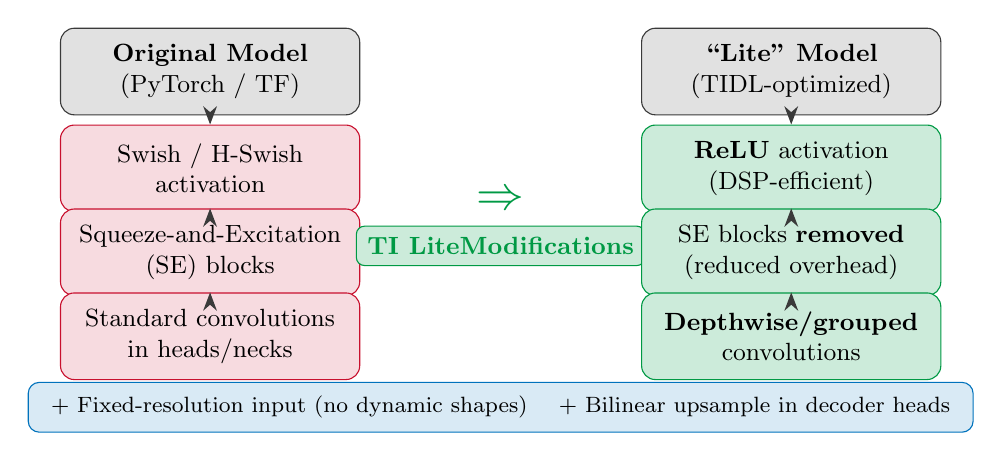
\begin{tikzpicture}[scale=0.82,
    box/.style={rounded corners=5pt, minimum width=3.8cm, minimum height=1.1cm,
                align=center, draw, font=\small, inner sep=5pt},
    arr/.style={->, >=Stealth, thick, TIDark}
  ]
    % Original model
    \node[box, fill=TIDark!15, draw=TIDark] (orig) at (-4.5, 2.5)
      {\textbf{Original Model}\\(PyTorch / TF)};

    \node[box, fill=TIRed!15, draw=TIRed] (swish) at (-4.5, 1.0)
      {Swish / H-Swish\\activation};

    \node[box, fill=TIRed!15, draw=TIRed] (se) at (-4.5, -0.3)
      {Squeeze-and-Excitation\\(SE) blocks};

    \node[box, fill=TIRed!15, draw=TIRed] (std) at (-4.5, -1.6)
      {Standard convolutions\\in heads/necks};

    \draw[arr] (orig) -- (swish);
    \draw[arr] (swish) -- (se);
    \draw[arr] (se) -- (std);

    % Arrow
    \node[font=\LARGE, TIGreen] at (0, 0.5) {$\Rightarrow$};
    \node[rounded corners=3pt, fill=TIGreen!20, draw=TIGreen,
          font=\small\bfseries, inner sep=4pt, text=TIGreen] at (0, -0.2)
      {TI Lite\\Modifications};

    % Lite model
    \node[box, fill=TIDark!15, draw=TIDark] (lite) at (4.5, 2.5)
      {\textbf{``Lite'' Model}\\(TIDL-optimized)};

    \node[box, fill=TIGreen!20, draw=TIGreen] (relu) at (4.5, 1.0)
      {\textbf{ReLU} activation\\(DSP-efficient)};

    \node[box, fill=TIGreen!20, draw=TIGreen] (nose) at (4.5, -0.3)
      {SE blocks \textbf{removed}\\(reduced overhead)};

    \node[box, fill=TIGreen!20, draw=TIGreen] (dw) at (4.5, -1.6)
      {\textbf{Depthwise/grouped}\\convolutions};

    \draw[arr] (lite) -- (relu);
    \draw[arr] (relu) -- (nose);
    \draw[arr] (nose) -- (dw);

    % Additional modifications
    \node[rounded corners=4pt, fill=TIBlue!15, draw=TIBlue,
          minimum width=12cm, inner sep=5pt, font=\footnotesize, align=center]
          at (0, -2.7)
      {+ Fixed-resolution input (no dynamic shapes) \quad
       + Bilinear upsample in decoder heads};
  \end{tikzpicture}
  \end{center}
\end{frame}

%--------------------------------------------------------------
\begin{frame}{Object Detection --- Selected Model Performance}
  \centering
  \scriptsize
  \begin{tabular}{lrlrrl}
    \toprule
    \textbf{Model} & \textbf{Input} & \textbf{Source} & \textbf{mAP\%} & \textbf{AP50\%} & \textbf{Format} \\
    \midrule
    \rowcolor{TIGray} YOLOX-nano-lite & 416px & edgeai-mmdet & 24.8 & 41.8 & ONNX \\
    YOLOX-tiny-lite & 416px & edgeai-mmdet & 32.0 & 50.7 & ONNX \\
    \rowcolor{TIGray} YOLOX-s-lite & 640px & edgeai-mmdet & 38.3 & 56.0 & ONNX \\
    YOLOX-m-lite & 640px & edgeai-mmdet & 44.8 & 63.0 & ONNX \\
    \rowcolor{TIGray} YOLOX-l-lite & 640px & edgeai-mmdet & 46.5 & 65.7 & ONNX \\
    \textbf{YOLOX-x-lite} & 640px & edgeai-mmdet & \textbf{50.6} & 68.9 & ONNX \\
    \rowcolor{TIGray} YOLOv7-l-lite & 640px & edgeai-mmdet & $\sim$50 & $\sim$68 & ONNX \\
    YOLOv9-s-lite & 640px & edgeai-mmdet & $\sim$46 & $\sim$63 & ONNX \\
    \rowcolor{TIGray} RTMDet-m-lite & 640px & edgeai-mmdet & $\sim$49 & $\sim$67 & ONNX \\
    DETR-ResNet50 & 768px & HuggingFace & 42.0 & 62.3 & ONNX \\
    \rowcolor{TIGray} SSD-MobileDetDSP & 320px & TF1 Garden & 28.9 & -- & TFLite \\
    SSD-ResNet50-FPN & 640px & TF2 Garden & 34.3 & -- & TFLite \\
    \rowcolor{TIGray} EfficientDet-lite0-ti-lite & 512px & AutoML & 33.6 & 53.3 & ONNX \\
    FCOS-r50-lite & 512px & edgeai-mmdet & $\sim$42 & -- & ONNX \\
    \bottomrule
  \end{tabular}
\end{frame}

%==============================================================
\section{Semantic Segmentation}
%==============================================================

\begin{frame}{Semantic Segmentation}
  \begin{columns}[T]
    \begin{column}{0.48\textwidth}
      \textbf{Task Setup}
      \begin{itemize}\footnotesize
        \item \textbf{Datasets:} ADE20K, Cityscapes, COCOSeg21, VOC2012, TI-RoboKit
        \item \textbf{Metric:} MeanIoU \%
        \item \textbf{Models:} \highlight{30+} models
        \item Dense per-pixel class prediction
      \end{itemize}

      \vspace{0.3cm}
      \begin{block}{Key Architectures}
        \begin{itemize}\scriptsize
          \item \textbf{DeepLabV3Lite} + MobileNetV2/V3
          \item \textbf{FPNLite} + MobileNetV2/RegNetX
          \item \textbf{UNetLite} + MobileNetV2
          \item \textbf{LR-ASPP} (torchvision)
          \item \textbf{SegFormer} B0/B5 (transformer)
          \item \textbf{DeepLabV3} Xception65 (TF)
          \item \textbf{QAT variants} (multiple)
        \end{itemize}
      \end{block}

      \vspace{0.2cm}
      \begin{alertblock}{QAT Segmentation}
        \scriptsize QAT models show only \textbf{$\sim$0.5 MeanIoU} drop vs FP32,
        demonstrating high quantization robustness for segmentation heads.
      \end{alertblock}
    \end{column}

    \begin{column}{0.48\textwidth}
      \begin{tikzpicture}
        \begin{axis}[
          xbar,
          title={\small Segmentation MeanIoU (selected)},
          xlabel={\scriptsize MeanIoU (\%)},
          symbolic y coords={
            {SegFormer-B0 ADE20K},
            {DeepLabV3Lite-MV2 ADE20K32},
            {DeepLabV3Lite-MV2 COCOSeg21},
            {LR-ASPP-MV3 COCOSeg21},
            {MV2+FPNLite COCOSeg21},
            {DeepLabV3-ResNet50 CityScapes},
            {RegNetX+FPNLite Cityscapes},
            {DeepLabV3-Xception65 Cityscapes}
          },
          ytick=data,
          yticklabel style={font=\tiny},
          xmin=30, xmax=90,
          width=6.5cm, height=6.2cm,
          tick label style={font=\tiny},
          label style={font=\scriptsize},
          title style={font=\scriptsize\bfseries},
          bar width=5pt,
          nodes near coords,
          nodes near coords style={font=\tiny},
          every node near coord/.append style={font=\tiny},
        ]
          \addplot[fill=TIBlue!70] coordinates {
            (37.4, {SegFormer-B0 ADE20K})
            (49.95, {DeepLabV3Lite-MV2 ADE20K32})
            (57.68, {DeepLabV3Lite-MV2 COCOSeg21})
            (57.9, {LR-ASPP-MV3 COCOSeg21})
            (58.12, {MV2+FPNLite COCOSeg21})
            (73.5, {DeepLabV3-ResNet50 CityScapes})
            (78.9, {RegNetX+FPNLite Cityscapes})
            (81.74, {DeepLabV3-Xception65 Cityscapes})
          };
        \end{axis}
      \end{tikzpicture}
    \end{column}
  \end{columns}
\end{frame}

%==============================================================
\section{Advanced Vision Tasks}
%==============================================================

\begin{frame}{Depth Estimation \& 3D Object Detection}
  \begin{columns}[T]
    \begin{column}{0.46\textwidth}
      \begin{block}{\faRulerCombined~Depth Estimation}
        \begin{itemize}\footnotesize
          \item \textbf{Dataset:} NYUDepthV2 (indoor RGBD)
          \item \textbf{Metric:} Delta1\% (predictions within 1.25× GT)
          \item Dense per-pixel depth map output
        \end{itemize}
      \end{block}

      \vspace{0.2cm}
      \footnotesize
      \begin{tabular}{lrrr}
        \toprule
        \textbf{Model} & \textbf{GMACs} & \textbf{Input} & \textbf{$\delta_1$\%} \\
        \midrule
        \rowcolor{TIGray} FastDepth & 0.38 & 224$^2$ & 77.1 \\
        MiDaS-small v2.1 & 4.63 & 256$^2$ & 86.67 \\
        \bottomrule
      \end{tabular}
    \end{column}

    \begin{column}{0.50\textwidth}
      \begin{block}{\faCar~3D Object Detection (BEV)}
        \begin{itemize}\footnotesize
          \item \textbf{Dataset:} PandaSet (camera BEV, 12 classes)
          \item \textbf{Metric:} mAP, NDS
          \item Bird's-Eye-View (BEV) camera-based approach
        \end{itemize}
      \end{block}

      \vspace{0.2cm}
      \scriptsize
      \begin{tabular}{lrrrr}
        \toprule
        \textbf{Model} & \textbf{Frames} & \textbf{Input} & \textbf{mAP} & \textbf{NDS} \\
        \midrule
        \rowcolor{TIGray} FastBEV-r18-f1 & 1 & 256$\times$704 & 17.5\% & 23.0\% \\
        FastBEV-r34-f4 & 4 & 256$\times$704 & 23.1\% & 29.5\% \\
        \rowcolor{TIGray} BEVFormer-tiny & 1 & 544$\times$960 & 23.0\% & 29.5\% \\
        PointPillars & -- & 496$\times$432 & \multicolumn{2}{c}{\textit{deprecated}} \\
        \bottomrule
      \end{tabular}

      \vspace{0.2cm}
      \begin{alertblock}{\scriptsize KITTI LiDAR}
        \scriptsize PointPillars (KITTI LiDAR) is \textbf{deprecated}.
        Camera BEV is the active direction.
      \end{alertblock}
    \end{column}
  \end{columns}
\end{frame}

%--------------------------------------------------------------
\begin{frame}{Keypoint Detection \& Pose Estimation}
  \begin{columns}[T]
    \begin{column}{0.48\textwidth}
      \textbf{Task Setup}
      \begin{itemize}\footnotesize
        \item \textbf{Dataset:} COCO Keypoints (17 human joints)
        \item \textbf{Metric:} AP @ [IoU 0.5:0.95]
        \item \textbf{Source:} edgeai-mmpose (TI fork of MMPose)
        \item Heatmap-free \textbf{single-stage approach}
        \item Detect + estimate pose in one forward pass
      \end{itemize}

      \vspace{0.3cm}
      \begin{tabular}{lrr}
        \toprule
        \textbf{Model} & \textbf{Input} & \textbf{AP\%} \\
        \midrule
        \rowcolor{TIGray} YOLOXPose-tiny-lite & 416$^2$ & 47.2 \\
        \textbf{YOLOXPose-s-lite} & 640$^2$ & \textbf{56.4} \\
        \rowcolor{TIGray} YOLOX-s-pose-ti-lite & 640$^2$ & 51.2 \\
        \bottomrule
      \end{tabular}

      \vspace{0.3cm}
      \begin{block}{6D Pose Estimation}
        \begin{itemize}\scriptsize
          \item \textbf{Dataset:} YCB-Video (21 household objects)
          \item \textbf{Model:} YOLOX-s-object-pose-ti-lite
          \item \textbf{Input:} 640×480, AP \textbf{AR=64.73\%}, ADD(s)=54.12\%
          \item End-to-end: RGB → 6-DOF pose (no post-processing on CPU)
        \end{itemize}
      \end{block}
    \end{column}

    \begin{column}{0.48\textwidth}
      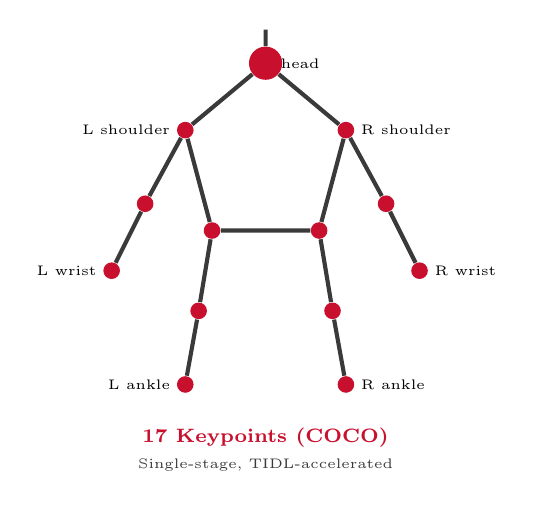
\begin{tikzpicture}[scale=0.85]
        % Skeleton diagram (simplified human pose)
        \tikzset{
          joint/.style={circle, fill=TIRed, minimum size=6pt, inner sep=0},
          bone/.style={TIDark, line width=1.5pt}
        }

        % Head
        \node[joint, minimum size=12pt] (head) at (3, 5.5) {};
        \node[font=\tiny, right=2pt] at (head) {head};

        % Shoulders
        \node[joint] (lsho) at (1.8, 4.5) {};
        \node[joint] (rsho) at (4.2, 4.5) {};
        \node[font=\tiny, left=2pt] at (lsho) {L shoulder};
        \node[font=\tiny, right=2pt] at (rsho) {R shoulder};

        % Elbows
        \node[joint] (lelb) at (1.2, 3.4) {};
        \node[joint] (relb) at (4.8, 3.4) {};

        % Wrists
        \node[joint] (lwri) at (0.7, 2.4) {};
        \node[joint] (rwri) at (5.3, 2.4) {};
        \node[font=\tiny, left=2pt] at (lwri) {L wrist};
        \node[font=\tiny, right=2pt] at (rwri) {R wrist};

        % Hips
        \node[joint] (lhip) at (2.2, 3.0) {};
        \node[joint] (rhip) at (3.8, 3.0) {};

        % Knees
        \node[joint] (lkne) at (2.0, 1.8) {};
        \node[joint] (rkne) at (4.0, 1.8) {};

        % Ankles
        \node[joint] (lank) at (1.8, 0.7) {};
        \node[joint] (rank) at (4.2, 0.7) {};
        \node[font=\tiny, left=2pt] at (lank) {L ankle};
        \node[font=\tiny, right=2pt] at (rank) {R ankle};

        % Bones
        \draw[bone] (head) -- (lsho) -- (lelb) -- (lwri);
        \draw[bone] (head) -- (rsho) -- (relb) -- (rwri);
        \draw[bone] (lsho) -- (lhip) -- (rhip) -- (rsho);
        \draw[bone] (lhip) -- (lkne) -- (lank);
        \draw[bone] (rhip) -- (rkne) -- (rank);
        \draw[bone] (head) -- ++(0, 0.5);

        \node[font=\scriptsize\bfseries, TIRed] at (3, -0.1) {17 Keypoints (COCO)};
        \node[font=\tiny, TIDark] at (3, -0.5) {Single-stage, TIDL-accelerated};
      \end{tikzpicture}
    \end{column}
  \end{columns}
\end{frame}

%==============================================================
\section{Model Formats \& Runtimes}
%==============================================================

\begin{frame}{Model Formats \& Inference Runtimes}
  \begin{center}
  \begin{tikzpicture}[scale=0.88,
    stage/.style={rounded corners=6pt, minimum width=3.2cm, minimum height=1.2cm,
                  align=center, draw, thick, font=\small\bfseries, drop shadow},
    arr/.style={->, >=Stealth, very thick}
  ]
    % Training frameworks
    \node[stage, fill=TIBlue!20, draw=TIBlue] (pytorch) at (-5.5, 3)
      {PyTorch /\\MMDetection};
    \node[stage, fill=TIBlue!15, draw=TIBlue!70] (tf) at (-5.5, 1.2)
      {TensorFlow\\(TF1 / TF2)};
    \node[stage, fill=TIBlue!10, draw=TIBlue!50] (mxnet) at (-5.5, -0.6)
      {MXNet /\\GluonCV};

    % Export formats
    \node[stage, fill=TIOrange!20, draw=TIOrange] (onnx) at (-1.5, 3)
      {\textbf{ONNX}\\(.onnx)};
    \node[stage, fill=TIOrange!15, draw=TIOrange!70] (tflite) at (-1.5, 1.2)
      {\textbf{TFLite}\\(.tflite)};

    % Runtimes
    \node[stage, fill=TIGreen!20, draw=TIGreen] (onr) at (2.0, 3.6)
      {\blue{ONR-}\\onnxrt};
    \node[stage, fill=TIGreen!15, draw=TIGreen!70] (tvm) at (2.0, 2.1)
      {\blue{TVM-}\\tvmrt/tvmdlr};
    \node[stage, fill=TIGreen!10, draw=TIGreen!50] (tfl) at (2.0, 0.6)
      {\blue{TFL-}\\tflitert};

    % TIDL
    \node[stage, fill=TIRed!25, draw=TIRed, minimum width=3.5cm,
          minimum height=1.4cm, font=\bfseries] (tidl) at (5.7, 2.1)
      {\textcolor{TIRed}{\faMicrochip}\\TIDL\\Accelerated};

    % SoC
    \node[stage, fill=TIDark!15, draw=TIDark, minimum width=3.5cm,
          minimum height=1.4cm] (soc) at (9.3, 2.1)
      {\textcolor{TIDark}{\faServer}\\TI SoC\\(MMA + C7x)};

    % Arrows: training → export
    \draw[arr, TIBlue] (pytorch) -- node[above, font=\tiny]{export} (onnx);
    \draw[arr, TIBlue!70] (tf) -- node[above, font=\tiny]{convert} (tflite);
    \draw[arr, TIBlue!50] (mxnet) -- (onnx);

    % Arrows: export → runtime
    \draw[arr, TIOrange] (onnx.east) -- (onr.west);
    \draw[arr, TIOrange!70] (onnx.east) -- (tvm.west);
    \draw[arr, TIOrange!50] (tflite.east) -- (tfl.west);

    % Arrows: runtime → TIDL → SoC
    \draw[arr, TIGreen] (onr.east) -- (tidl.west);
    \draw[arr, TIGreen!70] (tvm.east) -- (tidl);
    \draw[arr, TIGreen!50] (tfl.east) -- (tidl.west);
    \draw[arr, TIRed, very thick] (tidl) -- (soc);

  \end{tikzpicture}
  \end{center}
\end{frame}

%--------------------------------------------------------------
\begin{frame}{Pre-compiled Artifact Structure}
  \begin{columns}[T]
    \begin{column}{0.50\textwidth}
      \begin{block}{Artifact Naming Convention}
        \lstset{
          basicstyle=\ttfamily\scriptsize,
          breaklines=true,
          backgroundcolor=\color{TIGray},
          frame=single,
          framesep=3pt
        }
        \begin{lstlisting}
<RUNTIME>-<TASK>-<ID>-<description>

ONR-OD-8220-yolox-s-lite-coco-640x640
TFL-CL-0000-mobileNetV1-mlperf
TVM-SS-5720-deeplabV3-mobV2-512x512
        \end{lstlisting}
      \end{block}

      \vspace{0.3cm}
      \textbf{Task Abbreviations:}
      \begin{tabular}{ll}
        \texttt{CL} & Classification \\
        \texttt{OD} & Object Detection \\
        \texttt{SS} & Semantic Segmentation \\
        \texttt{KD} & Keypoint Detection \\
        \texttt{DE} & Depth Estimation \\
        \texttt{3DOD} & 3D Object Detection \\
        \texttt{6DPOSE} & 6D Pose Estimation \\
      \end{tabular}
    \end{column}

    \begin{column}{0.46\textwidth}
      \begin{block}{Artifact Bundle Contents}
        \begin{itemize}\footnotesize
          \item TIDL network files (compiled, SoC-specific)
          \item Calibration data files
          \item \texttt{param.yaml} (configuration)
          \item \texttt{extract.sh} (unpack helper)
        \end{itemize}
      \end{block}

      \vspace{0.3cm}
      \begin{block}{Directory Structure}
        \lstset{basicstyle=\ttfamily\scriptsize, backgroundcolor=\color{TIGray},
                frame=none}
        \begin{lstlisting}
modelartifacts/
  AM62A/8bits/
  AM67A/8bits/
  AM68A/8bits/  ← reference
  AM69A/8bits/
  TDA4VM/8bits/
        \end{lstlisting}
      \end{block}

      \vspace{0.2cm}
      \begin{exampleblock}{Metadata Files}
        \begin{itemize}\scriptsize
          \item \texttt{artifacts.yaml} — full metadata
          \item \texttt{artifacts.csv} — tabular lookup
          \item \texttt{shortlisted\_artifacts.yaml} — recommended quickstart set
        \end{itemize}
      \end{exampleblock}
    \end{column}
  \end{columns}
\end{frame}

%==============================================================
\section{Quantization}
%==============================================================

\begin{frame}{Quantization Strategy}
  \begin{columns}[T]
    \begin{column}{0.50\textwidth}
      \begin{block}{INT8 Quantization Targets}
        \begin{itemize}\footnotesize
          \item All deployed artifacts use \highlight{8-bit INT8}
          \item Typical CNN accuracy drop: \textbf{0.1–2\%}
          \item Transformer models: larger drop (e.g., Swin-tiny 82.1\% → 77.9\%)
          \item TIDL supports both PTQ and QAT paths
        \end{itemize}
      \end{block}

      \vspace{0.3cm}
      \textbf{Two quantization paths:}
      \begin{enumerate}\footnotesize
        \item \textbf{PTQ} (Post-Training Quantization)\\
              Via TIDL calibration dataset
        \item \textbf{QAT} (Quantization Aware Training)\\
              Suffix \texttt{-qat} or \texttt{-qat-p2} in model ID
      \end{enumerate}

      \vspace{0.3cm}
      \begin{alertblock}{QAT Accuracy (Classification)}
        \scriptsize
        \begin{tabular}{lrrl}
          \toprule
          Model & FP32 & QAT & $\Delta$ \\
          \midrule
          MobileNetV2 & 72.13 & 71.76 & $-$0.37 \\
          MobileNetV3Lite-L & 72.22 & 71.61 & $-$0.61 \\
          RegNetX-400MF & 73.81 & 73.38 & $-$0.43 \\
          \bottomrule
        \end{tabular}
      \end{alertblock}
    \end{column}

    \begin{column}{0.46\textwidth}
      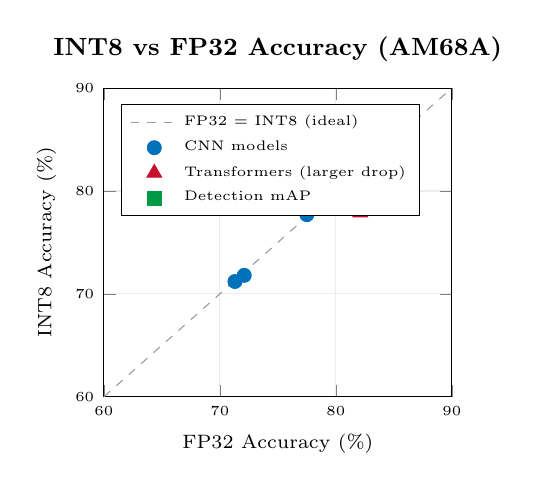
\begin{tikzpicture}
        \begin{axis}[
          title={\small INT8 vs FP32 Accuracy (AM68A)},
          xlabel={\scriptsize FP32 Accuracy (\%)},
          ylabel={\scriptsize INT8 Accuracy (\%)},
          xmin=60, xmax=90,
          ymin=60, ymax=90,
          width=6.0cm, height=5.5cm,
          grid=major, grid style={TIGray},
          tick label style={font=\tiny},
          label style={font=\scriptsize},
          title style={font=\scriptsize\bfseries},
          legend style={font=\tiny, at={(0.05,0.95)}, anchor=north west},
          legend cell align=left,
        ]
          % Ideal line y=x
          \addplot[dashed, TIDark!50, domain=60:90] {x};
          \addlegendentry{FP32 = INT8 (ideal)}

          % CNN points
          \addplot[only marks, mark=*, mark size=2.5pt, TIBlue]
            coordinates {
              (71.3, 71.2) (77.5, 77.7) (82.6, 82.4)
              (81.5, 81.3) (72.1, 71.8)
            };
          \addlegendentry{CNN models}

          % Transformer points (bigger drop)
          \addplot[only marks, mark=triangle*, mark size=3pt, TIRed]
            coordinates {
              (82.1, 77.9) (83.5, 81.2) (80.4, 79.1)
            };
          \addlegendentry{Transformers (larger drop)}

          % Detection
          \addplot[only marks, mark=square*, mark size=2.5pt, TIGreen]
            coordinates {
              (38.6, 38.2) (24.9, 24.6) (37.3, 37.0)
            };
          \addlegendentry{Detection mAP}
        \end{axis}
      \end{tikzpicture}
    \end{column}
  \end{columns}
\end{frame}

%==============================================================
\section{Accuracy Reports}
%==============================================================

\begin{frame}{Accuracy Reports \& Evaluation Framework}
  \begin{columns}[T]
    \begin{column}{0.50\textwidth}
      \begin{block}{Report Files}
        \begin{itemize}\footnotesize
          \item \texttt{reports/accuracy\_report\_20250307\_pc.md}
          \item \texttt{reports/accuracy\_report\_20250310\_pc.md}
          \item Format: Markdown + CSV
          \item Generated by \textbf{edgeai-benchmark} on PC emulation
        \end{itemize}
      \end{block}

      \vspace{0.3cm}
      \textbf{Report columns:}
      \begin{itemize}\scriptsize
        \item \texttt{model\_id}, \texttt{runtime\_name}, \texttt{task\_type}
        \item \texttt{dataset\_name}, \texttt{input\_resolution}
        \item \texttt{AM68A\_32bits-float-simulation\_metric} (FP32 baseline)
        \item \texttt{AM68A\_8bits\_metric} (INT8 deployed accuracy)
        \item \texttt{metric\_reference} (original training accuracy)
      \end{itemize}

      \vspace{0.3cm}
      \begin{alertblock}{Two Evaluation Modes}
        \begin{itemize}\scriptsize
          \item \textbf{Accuracy mode:} threshold=0.05, top\_k=500\\
                (comprehensive AP, maximizes accuracy score)
          \item \textbf{Performance mode:} threshold=0.3, top\_k=200\\
                (real-time deployment settings)
        \end{itemize}
      \end{alertblock}
    \end{column}

    \begin{column}{0.46\textwidth}
      \begin{tikzpicture}
        \begin{axis}[
          xbar,
          title={\small INT8 Accuracy: FP32 vs INT8 (Classification)},
          xlabel={\scriptsize Top-1 Accuracy (\%)},
          symbolic y coords={
            {MobileNetV1},
            {MobileNetV2},
            {EfficientNet-Lite4},
            {ResNet50},
            {Swin-tiny}
          },
          ytick=data,
          yticklabel style={font=\scriptsize},
          xmin=65, xmax=90,
          width=6.2cm, height=5.0cm,
          tick label style={font=\tiny},
          label style={font=\scriptsize},
          title style={font=\scriptsize\bfseries},
          bar width=7pt,
          legend style={font=\tiny, at={(0.98,0.05)}, anchor=south east},
          legend cell align=left,
        ]
          \addplot[fill=TIBlue!80] coordinates {
            (71.3, {MobileNetV1})
            (77.5, {MobileNetV2})
            (82.6, {EfficientNet-Lite4})
            (77.5, {ResNet50})
            (82.1, {Swin-tiny})
          };
          \addlegendentry{FP32}

          \addplot[fill=TIRed!80] coordinates {
            (71.2, {MobileNetV1})
            (71.8, {MobileNetV2})
            (82.4, {EfficientNet-Lite4})
            (77.7, {ResNet50})
            (77.9, {Swin-tiny})
          };
          \addlegendentry{INT8}
        \end{axis}
      \end{tikzpicture}
    \end{column}
  \end{columns}
\end{frame}

%==============================================================
\section{Datasets}
%==============================================================

\begin{frame}{Supported Datasets}
  \begin{columns}[T]
    \begin{column}{0.50\textwidth}
      \footnotesize
      \begin{tabular}{p{2.8cm}lp{2.2cm}}
        \toprule
        \textbf{Dataset} & \textbf{Task} & \textbf{Size} \\
        \midrule
        \rowcolor{TIGray} ImageNet-1K & Classification & 1.2M train / 50K val \\
        COCO 2017 & Det / Seg / KP & 118K / 5K val \\
        \rowcolor{TIGray} WIDER FACE & Face Detect. & 32K images \\
        ADE20K & Segmentation & 20K train \\
        \rowcolor{TIGray} Cityscapes & Segmentation & 3K fine-annot. \\
        VOC 2012 & Segmentation & 11K images \\
        \rowcolor{TIGray} NYUDepthV2 & Depth Est. & 1449 labeled \\
        KITTI & 3D Detection & ADAS benchmark \\
        \rowcolor{TIGray} PandaSet & 3D BEV & Autonomous driving \\
        YCB-Video & 6D Pose & RGB-D sequences \\
        \rowcolor{TIGray} TI-RoboKit & Seg (custom) & TI robotics kit \\
        CARLA (synthetic) & Visual Loc. & Synthetic driving \\
        \rowcolor{TIGray} MLPerf subsets & CL/OD/SS & Standardized \\
        \bottomrule
      \end{tabular}
    \end{column}

    \begin{column}{0.46\textwidth}
      \begin{tikzpicture}
        \pie[
          text=legend,
          color={TIRed!70, TIBlue!70, TIGreen!70, TIOrange!70,
                 TIDark!50, TILightBlue!70, TIRed!30},
          radius=2.0,
          style={font=\scriptsize}
        ]{
          22/ImageNet-1K,
          18/COCO 2017,
          15/ADE20K,
          15/Cityscapes,
          10/VOC 2012,
          10/NYUDepthV2,
          10/Others
        }
      \end{tikzpicture}
      \vspace{0.1cm}
      \begin{exampleblock}{\scriptsize MLPerf Benchmarks}
        \scriptsize The zoo includes standardized \textbf{MLPerf inference}
        baseline models for classification (MobileNetV1, ResNet50),
        detection (SSD-MobileNetV1), and segmentation (DeepLabV3).
      \end{exampleblock}
    \end{column}
  \end{columns}
\end{frame}

%==============================================================
\section{Ecosystem \& Toolchain}
%==============================================================

\begin{frame}{TI EdgeAI Development Ecosystem}
  \begin{tikzpicture}[scale=0.82,
    box/.style={rounded corners=6pt, minimum width=3.6cm, minimum height=1.1cm,
                align=center, draw, thick, font=\small\bfseries, drop shadow},
    arr/.style={->, >=Stealth, very thick, TIDark}
  ]
    % Training layer
    \node[box, fill=TIBlue!20, draw=TIBlue, minimum width=11cm] (train)
      at (0, 4.5)
      {Model Training Frameworks (edgeai-torchvision, edgeai-mmdetection, edgeai-mmpose, HuggingFace)};

    % Model Zoo
    \node[box, fill=TIRed!25, draw=TIRed, minimum width=5cm] (zoo)
      at (-2.0, 3.0)
      {\textcolor{TIRed}{\faDatabase}~\textbf{EdgeAI Model Zoo}\\180+ pre-trained models};

    % TIDL Tools
    \node[box, fill=TIOrange!20, draw=TIOrange, minimum width=5cm] (tidltools)
      at (3.5, 3.0)
      {\textcolor{TIOrange}{\faTools}~edgeai-tidl-tools\\ONNX/TFLite → TIDL compiler};

    % Benchmark
    \node[box, fill=TIGreen!20, draw=TIGreen] (bench)
      at (-3.5, 1.4)
      {\textcolor{TIGreen}{\faChartBar}~edgeai-benchmark\\Accuracy \& FPS measurement};

    % TIDLRunner
    \node[box, fill=TIGreen!15, draw=TIGreen!70] (runner)
      at (0.5, 1.4)
      {\textcolor{TIGreen!80}{\faTerminal}~edgeai-tidlrunner\\CLI compilation + benchmark};

    % Edge AI Studio
    \node[box, fill=TIBlue!15, draw=TIBlue!60] (studio)
      at (4.5, 1.4)
      {\textcolor{TIBlue}{\faGlobe}~Edge AI Studio\\Web GUI model selection};

    % SoCs
    \node[box, fill=TIDark!15, draw=TIDark, minimum width=11cm] (socs)
      at (0, -0.1)
      {TDA4VM~~AM62A~~AM67A~~AM68A~~AM69A~~(MMA + C7x DSP + ARM)};

    % Arrows
    \draw[arr] (train) -- (zoo);
    \draw[arr] (train) -- (tidltools);
    \draw[arr] (zoo) -- (bench);
    \draw[arr] (zoo) -- (runner);
    \draw[arr] (tidltools) -- (runner);
    \draw[arr] (bench) -- (socs);
    \draw[arr] (runner) -- (socs);
    \draw[arr] (studio) -- (socs);
  \end{tikzpicture}
\end{frame}

%--------------------------------------------------------------
\begin{frame}{Model ID Convention \& Scripts}
  \begin{columns}[T]
    \begin{column}{0.50\textwidth}
      \begin{block}{Model ID Structure}
        \lstset{basicstyle=\ttfamily\scriptsize, backgroundcolor=\color{TIGray},
                frame=single, framesep=3pt}
        \begin{lstlisting}
<task>-<id>

cl-6360     (onnxrt classifier)
od-8220     (onnxrt YOLOX detector)
ss-8610     (onnxrt segmenter)
kd-7060     (onnxrt keypoint)
de-7300     (onnxrt depth)
3dod-8140   (onnxrt BEV)
        \end{lstlisting}
      \end{block}

      \vspace{0.3cm}
      \textbf{ID Number Ranges:}
      \begin{itemize}\scriptsize
        \item \texttt{0000–2999} → \blue{tflitert} runtime
        \item \texttt{3000–5999} → \blue{tvmrt/tvmdlr} runtime
        \item \texttt{6000–9999} → \blue{onnxrt} runtime
      \end{itemize}
    \end{column}

    \begin{column}{0.46\textwidth}
      \begin{exampleblock}{Key Export Scripts}
        \begin{itemize}\scriptsize
          \item \texttt{export\_model\_torchvision.py}\\
                PyTorch TorchVision → ONNX
          \item \texttt{export\_model\_timm.py}\\
                TIMM models → ONNX
          \item \texttt{export\_model\_huggingface.py}\\
                HuggingFace → ONNX
          \item \texttt{tf2\_export\_classification.sh}\\
                TF2 classification → TFLite
          \item \texttt{tf2\_export\_detection.sh}\\
                TF2 detection → TFLite
          \item \texttt{onnx\_shape\_inference.py}\\
                ONNX shape inference pass
          \item \texttt{make\_link\_files.py}\\
                Generate .link pointer files
          \item \texttt{cleanup\_model\_files.py}\\
                Remove intermediate files
        \end{itemize}
      \end{exampleblock}
    \end{column}
  \end{columns}
\end{frame}

%==============================================================
\section{Device Compatibility \& Tutorials}
%==============================================================

%--------------------------------------------------------------
% SLIDE: Device Specs
%--------------------------------------------------------------
\begin{frame}{Compatible Devices --- Hardware Specifications}
  \centering
  \scriptsize
  \begin{tabular}{p{1.4cm}p{2.8cm}p{2.2cm}rp{2.0cm}p{2.2cm}}
    \toprule
    \textbf{SoC} & \textbf{CPU Cores} & \textbf{AI Accelerator} & \textbf{TOPS} & \textbf{EVM Board} & \textbf{SDK} \\
    \midrule
    \rowcolor{TIRed!15}
    \textbf{\textcolor{TIRed}{TDA4VM}} &
      2$\times$ A72 + 6$\times$ R5F + 2$\times$ C7x DSP + C66x &
      MMA (matrix accel.) & \textbf{8} &
      J721E EVM / TDA4VM SK &
      PROCESSOR-SDK-J721E \\[3pt]

    \rowcolor{TIBlue!10}
    \textbf{\textcolor{TIBlue}{AM62A}} &
      4$\times$ A53 + M4F &
      1$\times$ C7x + MMA & \textbf{1} &
      SK-AM62A-LP &
      EdgeAI SDK (PSDK Linux AM62A) \\[3pt]

    \rowcolor{TIBlue!18}
    \textbf{\textcolor{TIBlue!80}{AM67A}} &
      4$\times$ A53 + 2$\times$ R5F &
      1$\times$ C7x + MMA & \textbf{2} &
      SK-AM67A &
      EdgeAI SDK (PSDK Linux AM67A) \\[3pt]

    \rowcolor{TIGreen!12}
    \textbf{\textcolor{TIGreen}{AM68A}} &
      2$\times$ A72 + 6$\times$ R5F &
      2$\times$ C7x + MMA & \textbf{8} &
      SK-AM68A &
      EdgeAI SDK (PSDK Linux AM68A) \\[3pt]

    \rowcolor{TIOrange!12}
    \textbf{\textcolor{TIOrange}{AM69A}} &
      4$\times$ A72 + 8$\times$ R5F &
      4$\times$ C7x + MMA & \textbf{32} &
      SK-AM69A &
      EdgeAI SDK (PSDK Linux AM69A) \\
    \bottomrule
  \end{tabular}

  \vspace{0.35cm}
  \begin{columns}[T]
    \begin{column}{0.48\textwidth}
      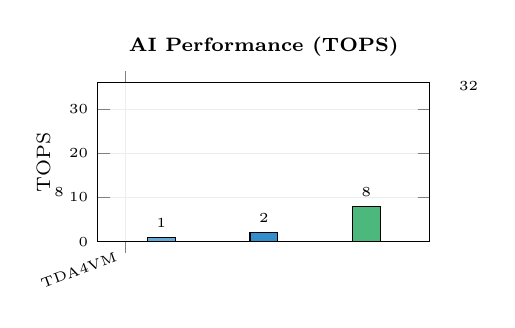
\begin{tikzpicture}
        \begin{axis}[
          title={\scriptsize AI Performance (TOPS)},
          symbolic x coords={TDA4VM, AM62A, AM67A, AM68A, AM69A},
          xtick=data,
          xticklabel style={font=\tiny, rotate=20, anchor=east},
          ymin=0, ymax=36,
          width=5.8cm, height=3.6cm,
          bar width=10pt,
          ybar,
          grid=major, grid style={TIGray},
          ylabel={\scriptsize TOPS},
          ylabel style={font=\scriptsize},
          title style={font=\scriptsize\bfseries},
          tick label style={font=\tiny},
          nodes near coords,
          nodes near coords style={font=\tiny\bfseries},
        ]
          \addplot[fill={TIRed!70}]   coordinates {(TDA4VM,8)};
          \addplot[fill={TIBlue!60}]  coordinates {(AM62A,1)};
          \addplot[fill={TIBlue!80}]  coordinates {(AM67A,2)};
          \addplot[fill={TIGreen!70}] coordinates {(AM68A,8)};
          \addplot[fill={TIOrange!80}]coordinates {(AM69A,32)};
        \end{axis}
      \end{tikzpicture}
    \end{column}
    \begin{column}{0.48\textwidth}
      \begin{block}{\scriptsize Key Shared Architecture}
        \begin{itemize}\scriptsize
          \item All SoCs run \textbf{TIDL} for DNN acceleration
          \item \textbf{MMA} handles convolution / matrix multiply
          \item \textbf{C7x DSP} handles activation, pooling, element-wise ops
          \item \textbf{ARM cores} handle pre/post-processing
          \item All support \textbf{INT8} inference from Model Zoo artifacts
        \end{itemize}
      \end{block}
    \end{column}
  \end{columns}
\end{frame}

%--------------------------------------------------------------
% SLIDE: Model-Device Compatibility Matrix
%--------------------------------------------------------------
\begin{frame}{Model--Device Compatibility Matrix}
  \centering
  \footnotesize

  \begin{tikzpicture}[scale=0.9,
    hdr/.style={fill=TIDark, text=white, font=\scriptsize\bfseries,
                inner sep=4pt, minimum height=0.55cm},
    cel/.style={inner sep=3pt, minimum height=0.55cm, minimum width=1.5cm,
                font=\scriptsize, align=center},
    yes/.style={cel, fill=TIGreen!25, text=TIGreen!80!black, font=\scriptsize\bfseries},
    par/.style={cel, fill=TIOrange!25, text=TIOrange!80!black, font=\scriptsize\bfseries},
    no/.style={cel,  fill=TIRed!15,   text=TIRed!60, font=\scriptsize},
  ]

    % Headers — SoCs
    \node[hdr, minimum width=3.2cm] at (0,    4.4) {Task / Model Family};
    \node[hdr, minimum width=1.6cm, fill=TIRed!80]   at (3.1,  4.4) {TDA4VM};
    \node[hdr, minimum width=1.6cm, fill=TIBlue!70]  at (4.75, 4.4) {AM62A};
    \node[hdr, minimum width=1.6cm, fill=TIBlue!85]  at (6.40, 4.4) {AM67A};
    \node[hdr, minimum width=1.6cm, fill=TIGreen!70] at (8.05, 4.4) {AM68A};
    \node[hdr, minimum width=1.6cm, fill=TIOrange!80]at (9.70, 4.4) {AM69A};

    % Row helper macro: \row{y}{label}{tda}{am62}{am67}{am68}{am69}
    % Using manual nodes for clarity
    \foreach \y/\lbl/\a/\b/\c/\d/\e in {
      3.70/{Classification (CNN)}/yes/yes/yes/yes/yes,
      3.05/{Classification (Transformer)}/par/no/par/yes/yes,
      2.40/{Object Detection (YOLOX)}/yes/par/yes/yes/yes,
      1.75/{Object Detection (DETR)}/par/no/par/yes/yes,
      1.10/{Semantic Segmentation}/yes/yes/yes/yes/yes,
      0.45/{Depth Estimation}/yes/yes/yes/yes/yes,
      -0.20/{Keypoint / Pose}/yes/par/yes/yes/yes,
      -0.85/{3D Detection (BEV)}/par/no/par/yes/yes,
      -1.50/{6D Pose Estimation}/yes/par/yes/yes/yes
    }{
      \node[cel, text=TIDark, minimum width=3.2cm, fill=TIGray, align=left,
            inner sep=4pt] at (0, \y) {\lbl};
      \node[\a, minimum width=1.6cm] at (3.1,  \y) {$\checkmark$};
      \node[\b, minimum width=1.6cm] at (4.75, \y)
        {\ifx\b yes$\checkmark$\else\ifx\b par\textasciitilde\else$\times$\fi\fi};
      \node[\c, minimum width=1.6cm] at (6.40, \y)
        {\ifx\c yes$\checkmark$\else\ifx\c par\textasciitilde\else$\times$\fi\fi};
      \node[\d, minimum width=1.6cm] at (8.05, \y)
        {\ifx\d yes$\checkmark$\else\ifx\d par\textasciitilde\else$\times$\fi\fi};
      \node[\e, minimum width=1.6cm] at (9.70, \y)
        {\ifx\e yes$\checkmark$\else\ifx\e par\textasciitilde\else$\times$\fi\fi};
    }

    % Legend
    \node[yes, rounded corners=3pt, draw=TIGreen!50] at (3.1,  -2.25) {$\checkmark$ Full support};
    \node[par, rounded corners=3pt, draw=TIOrange!50] at (6.40, -2.25) {\textasciitilde\ Limited / high-end models only};
    \node[no,  rounded corners=3pt, draw=TIRed!40]   at (9.70, -2.25) {$\times$ Not recommended};
  \end{tikzpicture}
\end{frame}

%--------------------------------------------------------------
% SLIDE: Recommended Models Per Device
%--------------------------------------------------------------
\begin{frame}{Recommended Model Configurations Per Device}
  \scriptsize
  \begin{tabular}{p{1.5cm}p{1.5cm}p{3.4cm}p{3.4cm}p{2.2cm}}
    \toprule
    \textbf{SoC} & \textbf{TOPS} & \textbf{Recommended Models} & \textbf{Use Case} & \textbf{Typical FPS} \\
    \midrule
    \rowcolor{TIRed!12}
    \textcolor{TIRed}{\textbf{TDA4VM}} & 8 &
      YOLOX-s/m-lite, FPNLite-Seg, MobileNetV2, FastBEV-r18 &
      ADAS: object detect + lane seg & 30--60 FPS \\[3pt]

    \rowcolor{TIBlue!10}
    \textcolor{TIBlue}{\textbf{AM62A}} & 1 &
      MobileNetV3Lite-Small/Large, YOLOX-nano-lite, DeepLabV3Lite-MV2 &
      Low-power edge: classify + light detection & 10--30 FPS \\[3pt]

    \rowcolor{TIBlue!18}
    \textcolor{TIBlue!80}{\textbf{AM67A}} & 2 &
      MobileNetV2, YOLOX-tiny-lite, FPNLite-Seg, YOLOXPose-tiny &
      Industrial: detect + segment + pose & 20--45 FPS \\[3pt]

    \rowcolor{TIGreen!12}
    \textcolor{TIGreen}{\textbf{AM68A}} & 8 &
      YOLOX-l-lite, Swin-Tiny, SegFormer-B0, FastBEV-r34, YOLOXPose-s &
      Robotics / multi-camera AI & 30--60 FPS \\[3pt]

    \rowcolor{TIOrange!12}
    \textcolor{TIOrange}{\textbf{AM69A}} & 32 &
      Swin-Large, YOLOX-x-lite, RTMDet-l, BEVFormer-tiny, YOLOX-s-pose &
      High-throughput: all tasks simultaneously & 60+ FPS \\
    \bottomrule
  \end{tabular}

  \vspace{0.25cm}
  \begin{columns}[T]
    \begin{column}{0.48\textwidth}
      \begin{alertblock}{\scriptsize \faLightbulb~Selection Tip}
        \scriptsize Use \textbf{Edge AI Studio} (ti.com/tool/EDGE-AI-STUDIO)
        to interactively filter models by SoC, latency budget, and accuracy
        threshold --- no hardware needed for initial evaluation.
      \end{alertblock}
    \end{column}
    \begin{column}{0.48\textwidth}
      \begin{exampleblock}{\scriptsize \faCloud~No Hardware? Use EVM Cloud}
        \scriptsize TI's \textbf{EVM Cloud/Farm} at \texttt{dev.ti.com/edgeai}
        lets you run compiled artifacts on real TI hardware remotely
        --- no EVM board required.
      \end{exampleblock}
    \end{column}
  \end{columns}
\end{frame}

%--------------------------------------------------------------
% SLIDE: Three Deployment Paths
%--------------------------------------------------------------
\begin{frame}{Three Paths to Deploy Models on TI Hardware}
  \begin{tikzpicture}[scale=0.88,
    path/.style={rounded corners=7pt, minimum width=3.6cm, minimum height=3.8cm,
                 align=center, draw, thick, drop shadow, inner sep=6pt},
    step/.style={rounded corners=3pt, fill=white, draw=TIDark!40,
                 minimum width=3.0cm, inner sep=3pt, font=\scriptsize, align=center},
    arr/.style={->, >=Stealth, thick}
  ]
    % Path 1: Edge AI Studio (web)
    \node[path, fill=TIBlue!15, draw=TIBlue] (p1) at (-4.5, 0.5) {};
    \node[font=\small\bfseries, TIBlue] at (-4.5, 2.15)
      {\faGlobe~Path 1: Edge AI Studio};
    \node[step, fill=TIBlue!10] at (-4.5, 1.35) {Browse \& filter models\\by SoC + task};
    \node[step, fill=TIBlue!10] at (-4.5, 0.45) {View FPS / latency /\\accuracy tradeoffs};
    \node[step, fill=TIBlue!10] at (-4.5, -0.45) {Download compiled\\artifact (.tar.gz)};
    \node[font=\tiny\itshape, TIBlue] at (-4.5, -1.15) {ti.com/tool/EDGE-AI-STUDIO};

    % Path 2: edgeai-tidlrunner (CLI)
    \node[path, fill=TIGreen!15, draw=TIGreen] (p2) at (0, 0.5) {};
    \node[font=\small\bfseries, TIGreen] at (0, 2.15)
      {\faTerminal~Path 2: edgeai-tidlrunner};
    \node[step, fill=TIGreen!10] at (0, 1.35) {Clone edgeai-tidlrunner\\+ modelzoo configs};
    \node[step, fill=TIGreen!10] at (0, 0.45) {Run compile + benchmark\\(PC emulation or EVM)};
    \node[step, fill=TIGreen!10] at (0, -0.45) {Deploy compiled\\binary to EVM board};
    \node[font=\tiny\itshape, TIGreen] at (0, -1.15) {github.com/TexasInstruments/edgeai-tidlrunner};

    % Path 3: PSDK RTOS (full SDK)
    \node[path, fill=TIOrange!15, draw=TIOrange] (p3) at (4.5, 0.5) {};
    \node[font=\small\bfseries, TIOrange] at (4.5, 2.15)
      {\faMicrochip~Path 3: PROCESSOR-SDK-RTOS};
    \node[step, fill=TIOrange!10] at (4.5, 1.35) {Install PROCESSOR-SDK\\-J721E (TDA4VM)};
    \node[step, fill=TIOrange!10] at (4.5, 0.45) {Integrate TIDL runtime\\into RTOS application};
    \node[step, fill=TIOrange!10] at (4.5, -0.45) {Deploy full\\automotive pipeline};
    \node[font=\tiny\itshape, TIOrange] at (4.5, -1.15) {ti.com/tool/PROCESSOR-SDK-J721E};

    % Bottom bar
    \node[rounded corners=4pt, fill=TIDark, text=white, minimum width=12cm,
          inner sep=5pt, font=\scriptsize\bfseries] at (0, -2.1)
      {All three paths use the same pre-compiled INT8 artifacts from edgeai-modelzoo};
  \end{tikzpicture}
\end{frame}

%--------------------------------------------------------------
% SLIDE: Tutorial & Reference Links
%--------------------------------------------------------------
\begin{frame}{Tutorial \& Reference Links}
  \begin{columns}[T]
    \begin{column}{0.48\textwidth}

      \begin{block}{\faBook~Official Documentation}
        \begin{itemize}\scriptsize
          \item \textbf{EdgeAI Landing Page}\\
                \url{https://www.ti.com/edgeai}
          \item \textbf{Edge AI Studio (Model Selection Tool)}\\
                \url{https://www.ti.com/tool/EDGE-AI-STUDIO}
          \item \textbf{PROCESSOR-SDK-J721E (TDA4VM SDK)}\\
                \url{https://www.ti.com/tool/PROCESSOR-SDK-J721E}
          \item \textbf{PSDK-RTOS-J721E User Guide}\\
                {\tiny\url{https://software-dl.ti.com/jacinto7/esd/processor-sdk-rtos-jacinto7/latest/exports/docs/}}
          \item \textbf{EVM Cloud / Remote Hardware Farm}\\
                \url{https://dev.ti.com/edgeai}
        \end{itemize}
      \end{block}

      \vspace{0.2cm}
      \begin{block}{\faGraduationCap~TI Training Courses}
        \begin{itemize}\scriptsize
          \item \textbf{Jacinto 7 Processors in Automotive}\\
                \url{https://training.ti.com/jacinto7}
          \item \textbf{Jacinto 7 Software Overview}\\
                \url{https://training.ti.com/jacinto7-software}
          \item \textbf{TI YouTube: Jacinto 7 Video Series}\\
                {\tiny\url{https://www.youtube.com/playlist?list=PLISmVLHAZbTRkVcGm3Bkkzx7Z2vFsM_zb}}
        \end{itemize}
      \end{block}

    \end{column}

    \begin{column}{0.48\textwidth}

      \begin{exampleblock}{\faGithub~GitHub Repositories}
        \begin{itemize}\scriptsize
          \item \textbf{edgeai-modelzoo} (this repo)\\
                {\tiny\url{https://github.com/TexasInstruments/edgeai-modelzoo}}
          \item \textbf{edgeai-benchmark} (accuracy + FPS eval)\\
                {\tiny\url{https://github.com/TexasInstruments/edgeai-benchmark}}
          \item \textbf{edgeai-tidl-tools} (TIDL compiler + firmware)\\
                {\tiny\url{https://github.com/TexasInstruments/edgeai-tidl-tools}}
          \item \textbf{edgeai-tidlrunner} (CLI compile + benchmark)\\
                {\tiny\url{https://github.com/TexasInstruments/edgeai-tidlrunner}}
          \item \textbf{Supported SoCs List (readme\_sdk.md)}\\
                {\tiny\url{https://github.com/TexasInstruments/edgeai/blob/main/readme_sdk.md}}
          \item \textbf{edgeai-torchvision} (classification training)\\
                {\tiny\url{https://github.com/TexasInstruments/edgeai-torchvision}}
          \item \textbf{QAT Tutorial}\\
                {\tiny\url{https://github.com/TexasInstruments/edgeai-torchvision/blob/master/docs/pixel2pixel/Quantization.md}}
          \item \textbf{edgeai-mmdetection} (detection training)\\
                {\tiny\url{https://github.com/TexasInstruments/edgeai-mmdetection}}
        \end{itemize}
      \end{exampleblock}

    \end{column}
  \end{columns}
\end{frame}

%--------------------------------------------------------------
% SLIDE: Getting Started Step-by-Step
%--------------------------------------------------------------
\begin{frame}{Getting Started --- Step-by-Step Quickstart}
  \begin{tikzpicture}[scale=0.85,
    step/.style={rounded corners=6pt, minimum width=2.4cm, minimum height=1.5cm,
                 align=center, draw, thick, font=\small, inner sep=5pt, drop shadow},
    arr/.style={->, >=Stealth, very thick, TIDark}
  ]
    % Step nodes
    \node[step, fill=TIBlue!20, draw=TIBlue] (s1) at (-5.5, 1.5)
      {\textbf{1}\\\scriptsize Clone\\edgeai-modelzoo};

    \node[step, fill=TIBlue!15, draw=TIBlue!70] (s2) at (-2.8, 1.5)
      {\textbf{2}\\\scriptsize Run\\download script};

    \node[step, fill=TIOrange!20, draw=TIOrange] (s3) at (0, 1.5)
      {\textbf{3}\\\scriptsize Browse models\\in Edge AI Studio};

    \node[step, fill=TIGreen!20, draw=TIGreen] (s4) at (2.8, 1.5)
      {\textbf{4}\\\scriptsize Compile with\\edgeai-tidlrunner};

    \node[step, fill=TIRed!20, draw=TIRed] (s5) at (5.5, 1.5)
      {\textbf{5}\\\scriptsize Deploy to\\EVM board};

    \draw[arr] (s1) -- (s2);
    \draw[arr] (s2) -- (s3);
    \draw[arr] (s3) -- (s4);
    \draw[arr] (s4) -- (s5);

    % Detail boxes below each step
    \node[rounded corners=3pt, fill=TIGray, draw=TIDark!30,
          minimum width=2.4cm, inner sep=4pt,
          font=\tiny, align=center] at (-5.5, 0)
      {\texttt{git clone}\\\texttt{TexasInstruments/}\\\texttt{edgeai-modelzoo}};

    \node[rounded corners=3pt, fill=TIGray, draw=TIDark!30,
          minimum width=2.4cm, inner sep=4pt,
          font=\tiny, align=center] at (-2.8, 0)
      {\texttt{./run\_download}\\\texttt{\_modelartifacts}\\\texttt{.sh}};

    \node[rounded corners=3pt, fill=TIGray, draw=TIDark!30,
          minimum width=2.4cm, inner sep=4pt,
          font=\tiny, align=center] at (0, 0)
      {Filter by SoC,\\task, TOPS, FPS\\at ti.com/tool/\\EDGE-AI-STUDIO};

    \node[rounded corners=3pt, fill=TIGray, draw=TIDark!30,
          minimum width=2.4cm, inner sep=4pt,
          font=\tiny, align=center] at (2.8, 0)
      {Use modelzoo\\configs in\\edgeai-tidlrunner\\data/configs/};

    \node[rounded corners=3pt, fill=TIGray, draw=TIDark!30,
          minimum width=2.4cm, inner sep=4pt,
          font=\tiny, align=center] at (5.5, 0)
      {Flash artifact to\\SK-AM68A /\\SK-AM69A /\\J721E EVM};

    % No-HW shortcut
    \draw[arr, dashed, TIBlue!60, bend left=25]
      (s3.south) to node[below, font=\tiny\itshape, TIBlue]{No hardware? Use dev.ti.com/edgeai} (s5.south);

    % Bottom note
    \node[rounded corners=4pt, fill=TIDark!10, draw=TIDark!40,
          minimum width=13cm, inner sep=5pt, font=\scriptsize]
          at (0, -1.5)
      {\faBook~Full SDK docs:
       \texttt{software-dl.ti.com/jacinto7/esd/processor-sdk-rtos-jacinto7/latest/}
       \quad \faGithub~\texttt{TexasInstruments/edgeai}};
  \end{tikzpicture}
\end{frame}

%==============================================================
\section{Summary}
%==============================================================

\begin{frame}{Summary Statistics}
  \begin{columns}[T]
    \begin{column}{0.50\textwidth}
      \begin{tikzpicture}
        \begin{axis}[
          xbar,
          title={\small Model Count by Task},
          xlabel={\scriptsize Number of Models},
          symbolic y coords={
            {Visual Localization},
            {6D Pose},
            {Depth Estimation},
            {3D Detection},
            {Keypoint},
            {Segmentation},
            {Detection},
            {Classification}
          },
          ytick=data,
          yticklabel style={font=\scriptsize},
          xmin=0, xmax=95,
          width=6.0cm, height=6.0cm,
          tick label style={font=\tiny},
          label style={font=\scriptsize},
          title style={font=\scriptsize\bfseries},
          bar width=6pt,
          nodes near coords,
          nodes near coords style={font=\tiny},
        ]
          \addplot[fill=TIRed!80] coordinates {
            (1,  {Visual Localization})
            (1,  {6D Pose})
            (2,  {Depth Estimation})
            (4,  {3D Detection})
            (5,  {Keypoint})
            (30, {Segmentation})
            (50, {Detection})
            (80, {Classification})
          };
        \end{axis}
      \end{tikzpicture}
    \end{column}

    \begin{column}{0.46\textwidth}
      \begin{block}{Key Numbers}
        \begin{itemize}
          \item \highlight{180+ total models}
          \item \blue{8 vision tasks}
          \item \green{5 TI SoC targets}
          \item \highlight{2 model formats} (ONNX + TFLite)
          \item \blue{3 inference runtimes}
          \item \green{INT8 all artifacts}
          \item Version \textbf{11.2.0}
        \end{itemize}
      \end{block}

      \vspace{0.3cm}
      \begin{block}{GigaMAC Efficiency Range}
        \begin{itemize}\footnotesize
          \item \textbf{Min:} MobileNetV3Lite-S\\
                0.054 GMACs → 62.68\% Top-1
          \item \textbf{Embedded sweet spot:}\\
                $<$10 GMACs for real-time
          \item \textbf{Best detection efficiency:}\\
                YOLOX-nano @ 1.476 GMACs, 24.8\% mAP
          \item \textbf{Max accuracy:}\\
                Swin-Large @ 34.5 GMACs, 86.15\%
        \end{itemize}
      \end{block}
    \end{column}
  \end{columns}
\end{frame}

%--------------------------------------------------------------
\begin{frame}{Key Takeaways}
  \begin{columns}[T]
    \begin{column}{0.48\textwidth}
      \begin{alertblock}{\faCheckCircle~Strengths}
        \begin{itemize}\footnotesize
          \item Comprehensive multi-task coverage (8 tasks)
          \item Ready-to-run INT8 artifacts for 5 SoCs
          \item Strong accuracy retention after INT8 quantization (CNN: $<$2\% drop)
          \item Active model additions (YOLOv7, YOLOv9, RTMDet in 2025)
          \item Transformer support (Swin, ViT, DETR, BEVFormer)
          \item QAT models for minimal accuracy loss
          \item Full toolchain integration (TIDL + edgeai-benchmark)
        \end{itemize}
      \end{alertblock}
    \end{column}

    \begin{column}{0.48\textwidth}
      \begin{exampleblock}{\faLightbulb~Use Case Guidance}
        \begin{itemize}\footnotesize
          \item \textbf{ADAS / automotive:} TDA4VM + YOLOX-l-lite for detection; FastBEV for 3D
          \item \textbf{Industrial edge:} AM62A + MobileNetV2/EfficientNet-Lite for classification
          \item \textbf{Robotics:} AM68A + FPNLite-Seg + YOLOXPose
          \item \textbf{Highest accuracy:} AM69A + Swin-Large (classification)
          \item \textbf{Lowest power:} AM62A + MobileNetV3Lite-Small
        \end{itemize}
      \end{exampleblock}

      \vspace{0.3cm}
      \begin{block}{\faLink~Getting Started}
        \begin{itemize}\scriptsize
          \item Clone: \texttt{edgeai-modelzoo} on GitHub
          \item Run: \texttt{run\_download\_modelartifacts.sh}
          \item Explore: \textbf{Edge AI Studio} at ti.com/tool/EDGE-AI-STUDIO
          \item Benchmark: \texttt{edgeai-benchmark} framework
        \end{itemize}
      \end{block}
    \end{column}
  \end{columns}
\end{frame}

%--------------------------------------------------------------
% FINAL SLIDE
%--------------------------------------------------------------
\begin{frame}[plain]
  
\begin{tikzpicture}[remember picture, overlay]
    \fill[TIDark] (current page.south west) rectangle (current page.north east);
    \fill[TIRed, opacity=0.85]
      (current page.south west) rectangle
      ([yshift=2.5cm]current page.south east);
    \fill[TIBlue, opacity=0.25]
      ([xshift=-1cm]current page.north west) --
      ([xshift=6cm]current page.north west) --
      ([xshift=4cm]current page.south west) --
      ([xshift=-1cm]current page.south west) -- cycle;
  \end{tikzpicture}

  \vspace{0.5cm}
  \begin{center}
    {\color{white}\Huge\textbf{Thank You}}\\[0.5cm]
    {\color{TIGray}\large TI EdgeAI Model Zoo v11.2.0}\\[0.3cm]
    {\color{TIGray}\normalsize 180+ models $\cdot$ 8 tasks $\cdot$ 5 SoCs $\cdot$ INT8 ready}\\[0.8cm]

    
\begin{tikzpicture}
      \node[rounded corners=6pt, fill=TIBlue, text=white, inner sep=8pt,
            font=\small\bfseries, align=center]{
        \faGithub~TexasInstruments/edgeai-modelzoo \quad
        \faGlobe~ti.com/tool/EDGE-AI-STUDIO\\[3pt]
        \faCloud~dev.ti.com/edgeai \quad
        \faGraduationCap~training.ti.com/jacinto7
      };
    \end{tikzpicture}\\[0.4cm]

    {\color{TIGray}\footnotesize
    Supported SoCs: TDA4VM $\cdot$ AM62A $\cdot$ AM67A $\cdot$ AM68A $\cdot$ AM69A
    (1--32 TOPS, INT8 artifacts ready)\\
    SDK: PROCESSOR-SDK-J721E $\cdot$ EdgeAI SDK (PSDK Linux AM6xA family)}
  \end{center}
\end{frame}

%==============================================================
\end{document}
%==============================================================
